\documentclass[conference]{IEEEtran}
\IEEEoverridecommandlockouts
% The preceding line is only needed to identify funding in the first footnote. If that is unneeded, please comment it out.
\usepackage{cite}
\usepackage{amsmath,amssymb,amsfonts}
\usepackage{algorithmic}
\usepackage{graphicx}
\usepackage{textcomp}
\usepackage{xcolor}
\usepackage{subcaption}
\def\BibTeX{{\rm B\kern-.05em{\sc i\kern-.025em b}\kern-.08em
    T\kern-.1667em\lower.7ex\hbox{E}\kern-.125emX}}
\begin{document}

\title{Formal Verification of an Asynchronous FIFO in SymbiYosys}

\author{\IEEEauthorblockN{Shidi Xi}
\IEEEauthorblockA{\textit{Department of Electrical and Computer Engineering} \\
\textit{The University of British Columbia}\\
Vancouver V6T 1Z4, Canada \\
xsd99@ece.ubc.ca}
}

\maketitle

\begin{abstract}
    yo
 \end{abstract}
 
 %\begin{IEEEkeywords}
 %    UVM, SVA, Verification, APB
 %\end{IEEEkeywords}
 
\section{Introduction}
Asynchronous FIFO is a hardware buffer that allows data to be written and read at different clock speeds. It is vital for preventing data loss or corruption when crossing clock domains. SymbiYosys is an open-source tool for hardware formal verification. Its verification process involves two methods. One methods is bounded model check (BMC), which is a technique that uses SAT or SMT solvers to check the correctness of a system within a predefined number of transitions. The second is k-induction. To prove system properties, it first demonstrates that they hold in a base case (the BMC), and then it checks for future steps via inductive reasoning. In this project, an asynchronous FIFO was designed in SystemVerilog and subsequently formally verified in SymbiYosys. Section description.
 
\section{ASYNCHRONOUS FIFO}
\subsection{IP Functionalities}
Figure \ref{fig:fifo} presents the schematic of the asynchronous FIFO designed in this project. Table \ref{tab:io} lists its IOs. In Figure \ref{fig:fifo}, there are 3 major components in the FIFO:

\begin{itemize}
    \item \textbf{Dual-port RAM}: Stores the data.
    \item \textbf{Write and read pointer handlers}: Controls the pointers, generates their Gray codes (\textit{g\_wptr} and \textit{g\_rptr}) and the \textit{full} and \textit{empty} flags.
    \item \textbf{Synchronizers}: Takes the write pointer in Gray code into the read clock domain and vice versa.
\end{itemize}

On positive edge of \textit{wclk}, if \textit{full} is 0, and \textit{w\_en} is 1, \textit{data\_in} will be written to the address indicated by the binary write pointer \textit{b\_wptr}, followed by its increment. \textit{data\_out} will always have the data at \textit{b\_rptr}, and on positive edge of \textit{rclk}, if \textit{empty} is 0 abd \textit{r\_en} is 1, a read transaction will complete and \textit{b\_rptr} will increment. The FIFO is empty when \textit{g\_rptr} equals \textit{g\_wptr\_sync} and is full when the two most significant
bits of \textit{g\_wptr} is the complement of \textit{g\_rptr\_sync} and the rest bits are equal.
 
\begin{figure}[h!]
    \centering
    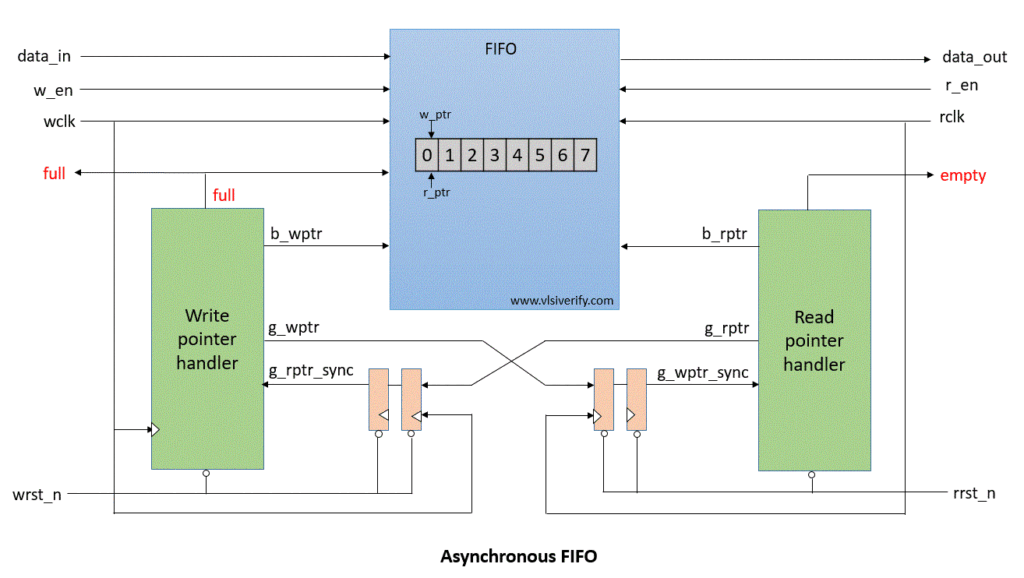
\includegraphics[width = 0.5\textwidth]{figures/asynchronous-fifo.png}
    \caption{Schematic of the asynchronous FIFO designed
    in this project (REF:https://vlsiverify.com/verilog/verilog-
    codes/asynchronous-fifo/).}
    \label{fig:fifo}
\end{figure}

\begin{table}[h!]
    \caption{List of IOs of the asynchronous FIFO.}
    \centering
    \begin{tabular}{|c c c c|}
        \hline
        Signal & I/O & Width & Description \\
        \hline
        wclk & Input & 1 & Write clock signal. \\
        wrst\_n & Input & 1 & Negative-high write reset signal. \\
        data\_in & Input & DATA\_WIDTH & Input data to be written.  \\
        w\_en & Input & 1 & Write enable. \\
        full & Input & 1 & Full flag. \\ 
        rclk & Input & 1 & Read clock signal. \\
        rrst\_n & Input & 1 & Negative-high read reset signal. \\
        data\_out & Input & DATA\_WIDTH & Output data to be read.  \\
        r\_en & Input & 1 & Read enable. \\
        empty & Input & 1 & Empty flag. \\ 
        \hline  
    \end{tabular}
    \label{tab:io}
\end{table}

\section{FORMAL VERIFICATION IN SYMBIYOSYS}
In SymbiYosys, formal verification can be either done using BMC or k-induction. Both methods require us to define the legal and the illegal states in our design.
\section{METHODOLOGY}

\section{Results}

\section{Conclusion}

%\bibliographystyle{IEEEtran}
%\bibliography{bibliography}

\end{document}